\section*{12. Bayesian Inference}\label{bayesian-inference}

\subsection*{12.1 Bayesian Philosophy}\label{bayesian-philosophy}
Postulates of \textbf{frequentist (or classical)} inference:
\begin{itemize}[tightlist]
\item
  Probabilty refers to limiting relative frequencies. Probabilities are
  objective properties of the real world.
\item
  Parameters are fixed, usually unknown constants. Because they are not
  fluctuating, no probability statements can be made about parameters.
\item
  Statistical procedures should be designed to have well defined long
  run frequency properties. For example, a 95\% confidence interval
  should trap the true value of the parameter with limiting frequency at
  least 95\%.
\end{itemize}
Postulates of \textbf{Bayesian} inference:
\begin{itemize}[tightlist]
\item
  Probability indicates degrees of belief, not limiting frequency. As
  such, we can make probability statements about lots of things, not
  just data which are subject to random variation. For example, I might
  say that `the probability that Albert Einstein drank a cup of tea on
  August 1 1948 is 35\%'. This does not refer to limiting frequency. It
  reflects my strength of belief that the proposition is true.
\item
  We can make probability statements about parameters, even though they
  are fixed constants.
\item
  We can make inferences about a parameter \(\theta\), by producing a
  probability distribution for \(\theta\). Inferences, such as point
  estimates and interval estimates, may then be extracted from this
  distribution.
\end{itemize}

\subsection*{12.2 The Bayesian Method}\label{the-bayesian-method}
Bayesian inference is usually carried out in the following way:
\begin{enumerate}[label={\arabic*.}]
\item
  Choose a probability density \(f(\theta)\) -- called the \textbf{prior
  distribution} -- that expresses our degrees of belief about a
  parameter \(\theta\) before we see any data.
\item
  We choose a statistical model \(f(x | \theta)\) that reflects our
  beliefs about \(x\) given \(\theta\).
\item
  After observing data \(X_{1}, \dots, X_{n}\), we update our beliefs and
  form the \textbf{posterior distribution}
  \(f(\theta | X_{1}, \dots, X_{n})\).
\end{enumerate}
Bayesian update:
\[
f(\theta | x^{n}) = \frac{f(x^{n} | \theta) f(\theta)}{\int f(x^{n} | \theta) f(\theta) d\theta} 
= \frac{\mathcal{L}_{n}(\theta) f(\theta)}{\int \mathcal{L}_{n} f(\theta) d\theta}
\propto \mathcal{L}_{n}(\theta) f(\theta)
\]
We throw away the denominator, which is a constant that does not depend
on \(\theta\), called a \textbf{normalizing constant}. We can summarize
this by writing:
\[
\text{"posterior is proportional to likelihood times prior"}
\]
We can obtain a \textbf{point estimate} using the posterior mean:
\[
\bar{\theta} = \int \theta f(\theta | x^{n}) d\theta = \frac{\int \theta \mathcal{L}_{n}(\theta) f(\theta)}{\int \mathcal{L}_{n}(\theta) f(\theta) d\theta}
\]
We can also obtain a Bayesian interval estimate. Define \(a\) and \(b\)
by 
\[
\int_{-\infty}^{a} f(\theta | x^{n}) d\theta =
\int_{b}^{\infty} f(\theta | x^{n}) d\theta = \alpha / 2.
\]
Let \(C = (a, b)\). Then
\[
\PROB(\theta \in C | x^{n}) = \int_a^{b} f(\theta | x^{n}) d\theta = 1 - \alpha
\]
so \textbf{\(C\) is a \(1 - \alpha\) posterior interval}.
When the prior and the posterior are in the same family, we say the
prior is \textbf{conjugate}.

\subsection*{12.3 Functions of
Parameters}\label{functions-of-parameters}
The posterior CDF for \(\tau = g(\theta)\) is
\[
H(\tau | x^{n}) = \PROB(g(\theta) \leq \tau) = \int_A f(\theta | x^{n}) d\theta
\]
where \(A = \{ \theta : g(\theta) \leq \tau \}\). The posterior density
is \(h(\tau | x^{n}) = H'(\tau | x^{n})\).

\subsection*{12.4 Simulation}\label{bayesian:simulation}
The posterior can often be approximated by simulation. Suppose we draw
\(\theta_{1}, \dots, \theta_B \sim p(\theta | x^{n})\). Then a histogram of
\(\theta_{1}, \dots, \theta_{n}\) approximates the posterior density
\(p(\theta | x^{n})\). An approximation to the posterior mean
\(\bar{\theta}_{n} = \EXP(\theta | x^{n})\) is
\(B^{-1} \sum_{j=1}^B \theta_{j}\). The posterior \(1 - \alpha\) interval
can be approximated by \((\theta_{\alpha/2}, \theta_{1 - \alpha/2})\)
where \(\theta_{\alpha/2}\) is the \(\alpha/2\) sample quantile of
\(\theta_{1}, \dots, \theta_B\).
Once we have a sample \(\theta_{1}, \dots, \theta_B\) from
\(f(\theta | x^{n})\), let \(\tau_{i} = g(\theta_{i})\). Then
\(\tau_{1}, \dots, \tau_B\) is a sample from \(f(\tau | x^{n})\). This
avoids the need to do analytical calculations. Simulation is discussed
in more detail later in the book.

\subsection*{12.5 Large Sample Properties for Bayes'
Procedures}\label{large-sample-properties-for-bayes-procedures}

\textbf{Theorem 12.5}. Under appropriate regularity conditions, we have
that the posterior is approximately
\(N(\hat{\theta}, \widehat{\SE}^{2})\) where \(\hat{\theta}_{n}\) is the
MLE and \(\widehat{\SE} = 1 / \sqrt{nI(\hat{\theta}_{n})}\). Hence,
\(\bar{\theta}_{n} \approx \hat{\theta}_{n}\). Also, if
\(C_{n} = (\hat{\theta}_{n} - z_{\alpha/2} \widehat{\SE}, \hat{\theta}_{n} + z_{\alpha/2} \widehat{\SE})\)
is the asymptotic frequentist \(1 - \alpha\) confidence interval, then
\(C_{n}\) is also an approximate \(1 - \alpha\) Bayesian posterior
interval:
\[
\PROB(\theta \in C_{n} | X^{n}) \rightarrow 1 - \alpha
\]
There is also a \textbf{Bayesian delta method}. Let
\(\tau = g(\theta)\). Then
\[
\tau | X^{n} \approx N(\hat{\tau}, \overline{\SE}^{2})
\]
where \(\hat{\tau} = g(\hat{\theta})\) and
\(\overline{\SE} = \SE | g'(\hat{\theta}) |\).

\subsection*{12.6 Flat Priors, Improper Priors and ``Noninformative''
Priors}\label{flat-priors-improper-priors-and-noninformative-priors}
\textbf{Improper priors}. We can adopt a flat prior
\(f(\theta) \propto c\) where \(c > 0\) is a constant. Note that
\(\int f(\theta) d\theta = \infty\) so this is not a real probability
density function in a proper sense. We call such prior an improper
prior. In general, improper priors are not a problem as long as the
resulting posterior is a well defined probability distribution.
\textbf{Flat priors are not invariant}. The notion of a flat prior is
not well-defined because a flat prior on a parameter does not imply a
flat prior ron a transformed version of a parameter.
\textbf{Jeffreys' prior}. Take \(f(\theta) \propto I(\theta)^{1/2}\)
where \(I(\theta)\) is the Fisher information function. This rule turns
out to be transformation invariant.
In a multiparameter problem, the Jeffreys' prior is defined to be
\(f(\theta) \propto \sqrt{\det I(\theta)}\), where
\(\det(A)\) denotes the determinant of a matrix \(A\).

\subsection*{12.7 Multiparameter
Problems}\label{multiparameter-problems}
Suppose that \(\theta = (\theta_{1}, \dots, \theta_p)\). The posterior
density is still given by
\[
p(\theta | x^{n}) \propto \mathcal{L}(\theta) f(\theta)
\]
Suppose we want to make inferences for \(\theta_{1}\). The marginal
posterior for \(\theta_{1}\) is
\[
f(\theta_{1} | x^{n}) = \int \cdots \int f(\theta_{1}, \dots, \theta_p) d\theta_{2} \dots d\theta_p
\]
In practice, it might not be feasible to do this integral. Simulation
can help. Draw randomly from the posterior:
\[
\theta^{1}, \dots, \theta^B \sim f(\theta | x^{n})
\]
where the superscripts index the different draws; each \(\theta^{j}\) is a
vector \(\theta^{j} = (\theta^{j}_{1}, \dots, \theta^{j}_p)\). Now collect
together the first component of each draw:
\[
\theta^{1}_{1}, \dots, \theta^B_{1}
\]
These form a sample from \(f(\theta_{1} | x^{n})\) and we have avoided doing
any integrals.

\subsection*{12.8 Strenghts and Weaknesses of Bayesian
Inference}\label{strenghts-and-weaknesses-of-bayesian-inference}
Frequentist and Bayesian methods are answering different questions:
\begin{itemize}[tightlist]
\item
  To combine prior beliefs with data in a principled way, use bayesian
  inference.
\item
  To construct procedures with guaranteed long run performance, such as
  confidence intervals, use frequentist methods.
\end{itemize}

\subsection*{12.9 Appendix}\label{appendix:bayesian}
\textbf{Proof of Theorem 12.5}.
It can be shown that the effect of the prior diminishes as \(n\)
increases so that
\(f(\theta | X^{n}) \propto \mathcal{L}_{n}(\theta)f(\theta) \approx \mathcal{L}_{n}(\theta)\).
Hence, \(\log f(\theta | X^{n}) \approx \ell(\theta)\). Now,
\(\ell(\theta) \approx \ell(\hat{\theta}) + (\theta - \hat{\theta})\ell'(\hat{\theta}) + [(\theta - \hat{\theta})^{2}/2]\ell''(\hat{\theta}) = \ell(\hat{\theta}) + [(\theta - \hat{\theta})^{2}/2] \ell''(\hat{\theta})\)
since \(\ell'(\hat{\theta}) = 0\). Exponentiating, we get approximately
that
\[
f(\theta | X^{n}) \propto \exp \left\{ - \frac{1}{2} \frac{(\theta - \hat{\theta})^{2}}{\sigma_{n}^{2}} \right\}
\]
where \(\sigma_{n}^{2} = 1 / \ell''(\hat{\theta}_{n})\). So the posterior of
\(\theta\) is approximately Normal with mean \(\hat{\theta}\) and
variance \(\sigma^{2}_{n}\). Let \(\ell_{i} = \log f(X_{i} | \theta)\), then
\begin{align*}
\sigma_{n}^{-2} &= -\ell''(\hat{\theta}_{n}) = \sum_{i} -\ell''_{i}(\hat{\theta}_{n}) \\
&= n \left( \frac{1}{n} \right) \sum_{i} -\ell''_{i}(\hat{\theta}_{n}) \approx n \EXP\left[-\ell''_{i}(\hat{\theta}_{n})\right] \\
&= n I(\hat{\theta}_{n})
\end{align*}
and hence \(\sigma_{n} \approx \SE (\hat{\theta})\).

\subsection*{12.11 Exercises}

\textbf{Exercise 12.11.1}. Verify (12.5).
\emph{Let \(X_{1}, \dots, X_{n} \sim N(\theta, \sigma^{2})\). For simplicity,
let us assume that \(\sigma\) is known. Suppose that we take as a prior
\(\theta \sim N(a, b^{2})\). In problem 1 of the homework, it is shown
that the posterior for \(\theta\) is}
\[
\theta | X^{n} \sim N(\bar{\theta}, \tau^{2})
\]
\emph{where}
\[
\bar{\theta} = w \bar{X} + (1 - w) a
\]
\emph{where}
\[
w = \frac{\frac{1}{\SE ^{2}}}{\frac{1}{\SE ^{2}} + \frac{1}{\text{b}^{2}}} \quad \text{and} \quad \frac{1}{\tau^{2}} = \frac{1}{\SE ^{2}} + \frac{1}{b^{2}}
\]
\emph{and \(\SE = \sigma / \sqrt{n}\) is the standard error of the
MLE \(\bar{X}\).}

\textbf{Solution}.
The posterior is proportional to the likelihood times the prior:
\[
p(\theta | x^{n}) \propto \mathcal{L}_{n}(\theta) f(\theta)
\]
The likelihood is the product of \(n\) Normal PDFs evaluated at
different data points:
\[
\mathcal{L}_{n}(\theta) = \prod_{i=1}^{n} f_X(X_{i}, \theta)
\]
Looking at the case \(n = 2\):
\begin{align*} 
f(X_{1}, \theta) f(X_{2}, \theta) &= 
\frac{1}{\sigma \sqrt{2 \pi}} \exp \left\{-\frac{1}{2} \left(\frac{X_{1} - \mu}{\sigma} \right)^{2} \right\}
\frac{1}{\sigma \sqrt{2 \pi}} \exp \left\{-\frac{1}{2} \left(\frac{X_{2} - \mu}{\sigma} \right)^{2} \right\} \\
&= \left( \frac{1}{\sigma \sqrt{2 \pi}} \right)^{2} \exp \left\{-\frac{1}{2\sigma^{2}} \left((X_{1} - \mu)^{2} + (X_{2} - \mu)^{2} \right) \right\} \\
&= \left( \frac{1}{\sigma \sqrt{2 \pi}} \right)^{2} \exp \left\{-\frac{1}{2\sigma^{2}} \left(
X_{1}^{2} + 2 X_{1} X_{2} + X_{2}^{2} - 2 (X_{1} + X_{2})\mu + 2\mu^{2} - 2 X_{1} X_{2}
\right) \right\} \\
&= \left( \frac{1}{\sigma \sqrt{2 \pi}} \right)^{2} \exp \left\{-\frac{1}{\sigma^{2}}\left(
\left(\mu - \frac{X_{1} + X_{2}}{2}\right)^{2} + \left(\frac{X_{1} + X_{2}}{2}\right)^{2} - X_{1} X_{2}
\right) \right\} \\
&= \left( \frac{1}{\sigma \sqrt{2 \pi}} \right)^{2} \exp \left\{-\frac{1}{2} \left(
\frac{\left(\mu - \frac{X_{1} + X_{2}}{2}\right)^{2} + \left(\frac{X_{1} + X_{2}}{2}\right)^{2} - X_{1} X_{2}}{\sigma^{2} / 2}
\right) \right\} \\
&= \left( \frac{1}{\sigma \sqrt{2 \pi}} \right)^{2} \exp \left\{-\frac{1}{2} \left(
\frac{\left(\mu - \frac{X_{1} + X_{2}}{2}\right)^{2}}{\sigma^{2} / 2} + C
\right) \right\} \\
&\propto \exp \left\{-\frac{1}{2}
\left(\frac{\mu - \frac{X_{1} + X_{2}}{2}}{\sigma / \sqrt{2}}\right)^{2}
\right\}
\end{align*}
The exponent is a quadratic form in \(\mu\), and that makes this
expression is proportional to the PDF of a Normal with mean \(\mu\) and
standard error \(\sigma / \sqrt{2}\), observed at the mean,
\(X = (X_{1} + X_{2})/2\).
This strongly suggests that, for the general case, the product is
proportional to the PDF of a Normal with mean \(\mu\) and standard error
\(\sigma / \sqrt{n}\), observed at the mean,
\(X = n^{-1} \sum_{i=1}^{n} X_{i}\). We can prove it by induction, going
through similar steps:
\begin{align*} 
f((X_{1}, \dots, X_{n}), \theta_{n}) f(X_{n+1}, \theta) &= 
\frac{1}{\sigma_{n} \sqrt{2 \pi}} \exp \left\{-\frac{1}{2} \left(\frac{\bar{X}_{n} - \mu}{\sigma_{n}} \right)^{2} \right\}
\frac{1}{\sigma \sqrt{2 \pi}} \exp \left\{-\frac{1}{2} \left(\frac{X_{n+1} - \mu}{\sigma} \right)^{2} \right\} \\
&\propto \exp \left\{-\frac{1}{2} \left( \left(\frac{\bar{X}_{n} - \mu}{\sigma_{n}} \right)^{2} + \left(\frac{X_{n+1} - \mu}{\sigma} \right)^{2} \right) \right\} \\
&= \exp \left\{-\frac{1}{2} \left( n \left(\frac{\bar{X}_{n} - \mu}{\sigma} \right)^{2} + \left(\frac{X_{n+1} - \mu}{\sigma} \right)^{2} \right) \right\} \\
&= \exp \left\{-\frac{1}{2 \sigma^{2}} \left( n \left(\bar{X}_{n} - \mu\right)^{2} + \left(X_{n+1} - \mu \right)^{2} \right) \right\} \\
&\propto \exp \left\{-\frac{1}{2} \left( \frac{\mu - (n\bar{X}_{n} + X_{n+1})}{\sigma / \sqrt{n+1}} \right)^{2} \right\}
= \exp \left\{-\frac{1}{2}
\left(\frac{\mu - \bar{X}_{n+1}}{\sigma / \sqrt{n+1}}\right)^{2}
\right\}
\end{align*}
Finally, we just need to prove one final result -- that the product of
the likelihood and the prior, both of which are PDFs of normals, is
proportional to yet another normal, with the parameters given. The steps
are again similar -- except now we are completing the squares in
\(\theta\), rather than \(\mu\), as each PDF has distinct mean
(\(\bar{X}\) and \(a\)) and standard error (\(\SE \) and
\(b\)).
\begin{align*}
\mathcal{L}_{n}(\theta) f(\theta) 
&= \frac{1}{\SE \sqrt{2 \pi}} \exp \left\{-\frac{1}{2} \left(\frac{\bar{X} - \theta}{\SE }\right)^{2} \right\} \frac{1}{b \sqrt{2 \pi}} \exp \left\{-\frac{1}{2} \left( \frac{a - \theta}{b} \right)^{2} \right\} \\
& \propto \exp \left\{-\frac{1}{2} \left( \left(\frac{\bar{X} - \theta}{\SE }\right)^{2} + \left( \frac{a - \theta}{b} \right)^{2} \right) \right\} \\
& \propto \exp \left\{-\frac{1}{2} \left( \frac{\bar{\theta} - \theta}{\tau} \right)^{2} \right\}
\end{align*}
which is the desired result.
An \textbf{excruciatingly complete} derivation of the results used here
-- products of Normal PDFs are proportional to Normal PDFs -- and more
general versions of it can be seen in Bromiley, Paul. ``Products and
convolutions of Gaussian probability density functions.'' Tina-Vision
Memo 3.4 (2003): 1, which is available online.

\textbf{Exercise 12.11.2}. Let \(X_{1}, \dots, X_{n} \sim N(\mu, 1)\).
\textbf{(a)} Simulate a dataset (using \(\mu = 5\)) consisting of
\(n = 100\) observations.
\textbf{(b)} Take \(f(\mu) = 1\) and find the posterior density. Plot
the density.
\textbf{(c)} Simulate 1000 draws from the posterior. Plot a histogram of
the simulated values and compare the histogram to the answer in (b).
\textbf{(d)} Let \(\theta = e^\mu\). Find the posterior density for
\(\theta\) analytically and by simulation.
\textbf{(e)} Find a 95\% posterior interval for \(\theta\).
\textbf{(f)} Find a 95\% confidence interval for \(\theta\).

\textbf{Solution}.
\textbf{(a)}

\begin{python}
import numpy as np
from scipy.stats import norm
import matplotlib.pyplot as plt
n = 100
mu = 5
sigma = 1
X = norm.rvs(loc=mu, scale=sigma, size=n)
\end{python}
\textbf{(b)} The posterior is proportional to likelihood times the
prior:
\[
f(\mu | X^{n}) \propto \mathcal{L}_{n}(\mu) f(\mu) = \mathcal{L}_{n}(\mu)
\]
But the likelihood is the product of the PDFs for each data point:
\[
\mathcal{L}_{n}(\mu) = \prod_{i=1}^{n} f(X_{i}; \mu)
\]
We can plot this with ``brute force'' -- calculating this product for
each sample point -- or use the analytic result that the likelihood is
proportional to a random variable following a Normal distribution in
\(\mu\) with mean \(\hat{\mu} = \bar{X}\) and standard error
\(\sigma / \sqrt{n}\):
\[
\mathcal{L}_{n}(\mu) \propto N(\bar{X}, \sigma^{2} / n)
\]

\begin{python}
# posterior is proportional to likelihood times f(\mu)
# likelihood is \prod_{i} f(X_{i}; \mu)
# pdf is f(x; (\mu, \sigma^{2})), the density of the normal function
mu_hat = X.mean()
mu_values = np.linspace(4, 6, 100)
\end{python}

\begin{python}
# Brute-force solution: explicitly compute the PDF for each sample, and multiply everything 
# (or take logs, add, and exponentiate):
likelihood = np.vectorize(lambda mu_hat: np.exp(np.log(norm.pdf(X, 
                                                loc=mu_hat,
                                                scale=sigma)).sum()))
L_i = likelihood(mu_values)
plt.plot(mu_values, L_i / L_i.sum())
\end{python}

\begin{figure}[H]
\centering
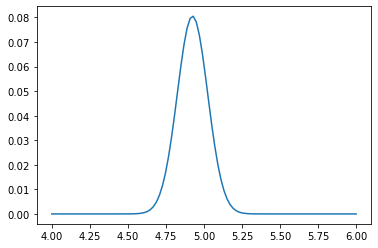
\includegraphics{Figure-12-01}
\end{figure}


\begin{python}
# Alternatively, use the analytic solution, \mathcal{L}_{n}(\mu) \sim N(\mu_hat, \sigma^{2}/n)
L_i2 = norm.pdf(mu_values, loc=mu_hat, scale=sigma/np.sqrt(n))
plt.plot(mu_values, L_i2 / L_i2.sum())
\end{python}

\begin{figure}[H]
\centering
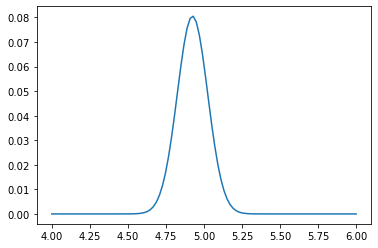
\includegraphics{Figure-12-02}
\end{figure}

\textbf{(c)}

\begin{python}
fig, (ax1,ax2) = plt.subplots(2, 1, sharex='col')
ax1.plot(mu_values, L_i2 / L_i2.sum())
posterior_samples = norm.rvs(loc=mu_hat, scale=sigma/np.sqrt(n), size=1000)
ax2.hist(posterior_samples, density=True, bins=mu_values)
\end{python}

\begin{figure}[H]
\centering
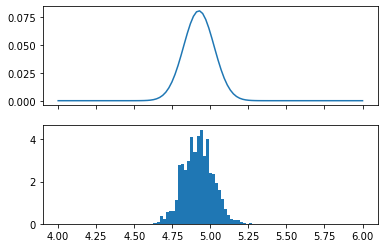
\includegraphics{Figure-12-03}
\end{figure}

\textbf{(d)}
Let \(Y = e^X\). Analytically:
\begin{itemize}[tightlist]
\item
  The CDF is
  \(F_Y(z) = \PROB_\theta(e^X \leq z) = \PROB_\mu(X \leq \log z) = \PROB_\mu \left( \frac{X - \mu}{\sigma} \leq \frac{\log z - \mu}{\sigma} \right) = \PROB(Z \leq \log z - \mu) = \Phi(\log z - \mu)\),
  where \(\Phi\) is the CDF of a standard normal distribution.
\item
  The PDF is
  \(f_Y(z) = F'_Y(z) = \partial \Phi(\log z - \mu) / \partial z = \phi(\log z - \mu) / z\),
  where \(\phi = \Phi'\) is the PDF of a standard normal function.
\end{itemize}

\begin{python}
def posterior_density(z):
    # Suppress warnings about log(z) when z < 0 and division by zero 
    # np.where will filter out invalid values
    with np.errstate(divide='ignore', invalid='ignore'):
        return np.where(z > 0, norm.pdf(np.log(z) - mu_hat) / z, 0)
    
z_values = np.linspace(0, 500, 100)
f_values = posterior_density(z_values)
plt.plot(z_values, f_values)
\end{python}

\begin{figure}[H]
\centering
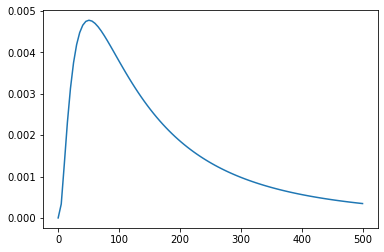
\includegraphics{Figure-12-04}
\end{figure}


\begin{python}
# By simulation:
# Resample from the estimated parametric distribution for X, and calculate Y = exp(X)
Y = np.exp(norm.rvs(loc=mu_hat, scale=sigma, size=10000))
# Recompute ranges for plot based on observed Y values
z_values = np.linspace(0, max(Y), 100)
f_values = posterior_density(z_values)
fig, (ax1,ax2) = plt.subplots(2, 1, sharex='col')
ax1.plot(z_values, f_values)
ax2.hist(Y, density=True, bins=z_values)
\end{python}

\begin{figure}[H]
\centering
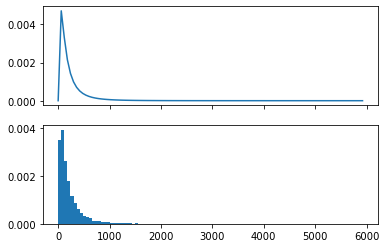
\includegraphics{Figure-12-05}
\end{figure}

\textbf{(e)}
Analytic solution: \(Y = g(X) = e^X\) and \(X \sim N(\mu, 1)\). Since
\(g\) is a monotonically increasing function, the quantiles of \(Y\) are
the exponentials of the quantiles of \(X\); that is,
\[
F_Y^{-1}(q) = g(F_X^{-1}(q)) = e^{F_X^{-1}(q)}
\]
But \(X\) follows a Normal distribution -- we can plug in the MLE for
\(\mu\), \(\hat{\mu} = \bar{X}\), obtain the quantiles for \(X\),
and then obtain the quantiles for \(Y\).
\begin{align*}
F_X^{-1}(q) &= \Phi^{-1}(q) / \sigma + \mu \\
F_Y^{-1}(q) &= e^{\Phi^{-1}(q) / \sigma + \mu}
\end{align*}

\begin{python}
from scipy.stats import norm
z_025 = norm.ppf(0.025)
z_975 = norm.ppf(0.975)
posterior_interval_analytic = (np.exp(z_025 + mu_hat), np.exp(z_975 + mu_hat))
print("95%% posterior interval (analytic):  %.3f, %.3f" % posterior_interval_analytic)
\end{python}
\begin{console}
95\% posterior interval (analytic):  19.388, 977.081
\end{console}
Alternatively, we can just sample from our simulation draws to get an
approximation:

\begin{python}
# Find percentile from simulated draws
posterior_interval_simulation = (
    np.quantile(Y, 0.025),
    np.quantile(Y, 0.975)
)
print("95%% posterior interval (simulation):  %.3f, %.3f" % posterior_interval_simulation)
\end{python}
\begin{console}
95\% posterior interval (simulation):  19.021, 985.730
\end{console}
\textbf{(f)}
For the Bayesian interval estimate, we need to find \(C = (a, b)\) such
that
\[
\int_{-\infty}^{a} f_Y(\theta | X^{n}) d\theta = \int_b^{\infty} f_Y(\theta | X^{n}) d\theta = \frac{\alpha}{2}
\]
or, using the cumulative density functions,
\[
F_Y(a) = 1 - F_Y(b) = \frac{\alpha}{2}
\]
\[
\Phi(\log a - \mu) = 1 - \Phi(\log b - \mu) = \frac{\alpha}{2}
\]
Solving for \(a\) and \(b\),
\[
a = e^{\mu + \Phi^{-1}(\alpha / 2)}
\quad \text{and} \quad
b = e^{\mu + \Phi^{-1}(1 - \alpha / 2)}
\]
This is exactly the same calculation as the analytic solution for the
posterior interval.

\begin{python}
from scipy.stats import norm
z_025 = norm.ppf(0.025)
z_975 = norm.ppf(0.975)
confidence_interval_analytic = (np.exp(z_025 + mu_hat), np.exp(z_975 + mu_hat))
print("95%% confidence interval (analytic):  %.3f, %.3f" % confidence_interval_analytic)
\end{python}
\begin{console}
95\% confidence interval (analytic):  19.388, 977.081
\end{console}

\textbf{Exercise 12.11.3}. Let
\(X_{1}, \dots, X_{n} \sim \text{Uniform}(0, \theta)\). Let
\(f(\theta) \propto 1/\theta\). Find the posterior density.

\textbf{Solution}. The posterior density is proportional to the
likelihood times the prior:
\begin{align*}
f(\theta | X^{n}) &\propto \mathcal{L}_{n}(\theta) f(\theta) \\
&= \frac{1}{\theta} \prod_{i=1}^{n} f(X_{i}; \theta)  \\
&= \frac{1}{\theta} \prod_{i=1}^{n} \frac{I(X_{i} \leq \theta)}{\theta} \\
&= \theta^{-(n+1)} I( \max \{ X_{1}, \dots, X_{n} \} \leq \theta \} ) \\
&= \begin{cases}
\theta^{-(n+1)} & \text{if } \theta \geq \max \{ X_{1}, \dots, X_{n} \} \\
0 & \text{otherwise}
\end{cases}
\end{align*}
Now we just need to normalize the posterior density so it integrates to
1. Let \(m = \max \{ X_{1}, \dots, X_{n} \}\). Then:
\[
1 = \int_{-\infty}^{\infty} f(\theta) d\theta  = \int_m^{\infty} c \theta^{-(n+1)} d\theta = c m^{-n} / n
\]
Solving this we get \(c = n m^{n}\), so the posterior density is:
\[
f(\theta) = \begin{cases}
\frac{n}{\theta} \left(\frac{m}{\theta}\right)^{n} & \text{if } \theta \geq m \\
0 & \text{otherwise}
\end{cases}
\]
where \(m = \max \{ X_{1}, \dots, X_{n} \}\).

\textbf{Exercise 12.11.4}. Suppose that 50 people are given a placebo
and 50 are given a new treatment. 30 placebo patients show improvement
while 40 treated patients show improvement. Let \(\tau = p_{2} - p_{1}\)
where \(p_{2}\) is the probability of improving under treatment and
\(p_{1}\) is the probability of improving under placebo.
\textbf{(a)} Find the MLE of \(\tau\). Find the standard error and 90\%
confidence interval using the delta method.
\textbf{(b)} Find the standard error and 90\% confidence interval using
the parametric bootstrap.
\textbf{(c)} Use the prior \(f(p_{1}, p_{2}) = 1\). Use simulation to find
the posterior mean and posterior 90\% interval for \(\tau\).
\textbf{(d)} Let
\[
\psi = \log \left( \left( \frac{p_{1}}{1 - p_{1}} \div \frac{p2}{1 - p2} \right) \right)
\]
be the log-odds ratio. Note that \(\psi = 0\) if \(p_{1} = p_{2}\). Find the
MLE of \(\psi\). Use the delta method to find a 90\% confidence interval
for \(\psi\).
\textbf{(e)} Use simulation to find the posterior mean and posterior
90\% interval for \(\psi\).

\textbf{Solution}.
\textbf{(a)}
We have two random variables, \(X_{1} \sim \text{Binomial}(n_{1}, p_{1})\) and
\(X_{2} \sim \text{Binomial}(n_{2}, p_{2})\). We are given \(n_{1} = n_{2} = 50\),
and the measurements \(X_{1} = 30\) and \(X_{2} = 40\).
We wish to estimate \(\tau = g(p_{1}, p_{2}) = p_{2} - p_{1}\). The MLE is
simply
\(\hat{\tau} = g(\hat{p}_{1}, \hat{p}_{2}) = \hat{p}_{2} - \hat{p}_{1} = X_{2} / n_{2} - X_{1} / n_{1}\).
Using the multiparameter delta method, the gradient of \(g\) is
\[
\nabla g = 
\begin{pmatrix} \partial g / \partial p_{1} \\ \partial g / \partial p_{2} \end{pmatrix} 
= \begin{pmatrix} -1 \\ 1 \end{pmatrix} 
\]
The log likelihood is:
\begin{align*}
\ell(p_{1}, p_{2}) &= \log f_{X_{1}}(X_{1}; p_{1}) + \log f_{X_{2}}(X_{2}; p_{2}) \\
& = \log \binom{n_{1}}{X_{1}} p_{1}^{X_{1}} (1 - p_{1})^{n_{1} - X_{1}}
+ \log \binom{n_{2}}{X_{2}} p_{2}^{X_{2}} (1 - p_{2})^{n_{2} - X_{2}} \\
&= \log \binom{n_{1}}{X_{1}} + X_{1} \log p_{1} + (n_{1} - X_{1}) \log (1 - p_{1})
\\
& \quad 
+ \log \binom{n_{2}}{X_{2}} + X_{2} \log p_{2} + (n_{2} - X_{2}) \log (1 - p_{2}) \\
&= X_{1} \log p_{1} + (n_{1} - X_{1}) \log (1 - p_{1}) + X_{2} \log p_{2} + (n_{2} - X_{2}) \log (1 - p_{2}) + C
\end{align*}
where \(C\) does not depend on \(p_{1}\) or \(p_{2}\).
The partial derivatives of the log likelihood are:
\begin{align*}
\Frac{\partial^{2} \ell}{\partial p_{1}^{2}} & = - \Frac{X_{1}}{p_{1}^{2}} - \frac{n_{1} - X_{1}}{(1 - p_{1})^{2}} \\
\Frac{\partial^{2} \ell}{\partial p_{2}^{2}} & = - \Frac{X_{2}}{p_{2}^{2}} - \frac{n_{2} - X_{2}}{(1 - p_{2})^{2}} \\
\Frac{\partial^{2} \ell}{\partial p_{1} \partial p_{2}} & = 0
\end{align*}
The Fisher Information Matrix is
\[
I_{n}(p_{1}, p_{2}) = -\begin{pmatrix}
\EXP\left[ \Frac{\partial^{2} \ell}{\partial p_{1}^{2}} \right]
& \EXP\left[ \Frac{\partial^{2} \ell}{\partial p_{1} \partial p_{2}} \right]  \\
\EXP\left[ \Frac{\partial^{2} \ell}{\partial p_{1} \partial p_{2}} \right]
& \EXP\left[ \Frac{\partial^{2} \ell}{\partial p_{2}^{2}} \right]
\end{pmatrix} = \begin{pmatrix}
\Frac{n_{1}}{p_{1}(1 - p_{1})} & 0 \\
0 & \Frac{n_{2}}{p_{2}(1 - p_{2})}
\end{pmatrix}
\]
and its inverse is
\[
J_{n}(p_{1}, p_{2}) = I_{n}^{-1}(p_{1}, p_{2}) = 
\begin{pmatrix} 
\Frac{p_{1}(1 - p_{1})}{n_{1}} & 0 \\
0 & \Frac{p_{2}(1 - p_{2})}{n_{2}}
\end{pmatrix}
\]
Then,
\[
\widehat{\SE}(\hat{\tau}) = \sqrt{(\hat{\nabla}g)^T \hat{J}_{n} (\hat{\nabla}g)}
= \sqrt{\frac{\hat{p}_{1}(1 - \hat{p}_{1})}{n_{1}} + \frac{\hat{p}_{2}(1 - \hat{p}_{2})}{n_{2}}}
\]
And we get the confidence interval:
\[
\hat{\tau} \pm z_{1 - \alpha/2}\widehat{\SE}(\hat{\tau})
\]

\begin{python}
import numpy as np
from scipy.stats import norm
n1 = 50
n2 = 50
X1 = 30
X2 = 40
p1_hat = X1 / n1
p2_hat = X2 / n2
tau_hat = p2_hat - p1_hat
se_hat = np.sqrt((p1_hat * (1 - p1_hat) / n1) + (p2_hat * (1 - p2_hat) / n2))
z_90 = norm.ppf(0.95)
confidence_interval = (tau_hat - z_90 * se_hat, tau_hat + z_90 * se_hat)
print('Estimated difference of means: \t\t %.3f' % tau_hat)
print('Estimated 90%% confidence interval:\t %.3f, %.3f' % confidence_interval)
\end{python}
\begin{console}
Estimated difference of means:           0.200
Estimated 90\% confidence interval:       0.053, 0.347
\end{console}
\textbf{(b)}

\begin{python}
import numpy as np
from scipy.stats import binom
B = 100000
n1 = 50
n2 = 50
X1 = 30
X2 = 40
p1_hat = X1 / n1
p2_hat = X2 / n2
XX1 = binom.rvs(n1, p1_hat, size=B)
XX2 = binom.rvs(n2, p2_hat, size=B)
tau_boot = XX2 / n2 - XX1 / n1
tau_boot_hat = tau_boot.mean()
q_05 = np.quantile(tau_boot, 0.05)
q_95 = np.quantile(tau_boot, 0.95)
boot_confidence_interval = (q_05, q_95)
print('Estimated difference of means: \t\t %.3f' % tau_boot_hat)
print('Estimated 90%% confidence interval:\t %.3f, %.3f' % boot_confidence_interval)
\end{python}
\begin{console}
Estimated difference of means:           0.200
Estimated 90\% confidence interval:       0.060, 0.340
\end{console}
\textbf{(c)} The posterior density is proportional to the likelihood
times the prior:
\begin{align*}
f((p_{1}, p_{2}) | X^{2}) &\propto \mathcal{L}(p_{1}, p_{2} | X^{2}) f(p_{1}, p_{2}) \\
&= f_{X_{1}}(X_{1} | p_{1}) f_{X_{2}}(X_{2} | p_{1}) \cdot 1 \\
&= \binom{n_{1}}{X_{1}} p_{1}^{X_{1}} (1 - p_{1})^{n_{1} - X_{1}} \binom{n_{2}}{X_{2}} p_{2}^{X_{2}} (1 - p_{2})^{n_{2} - X_{2}} \\
&\propto p_{1}^{X_{1}} (1 - p_{1})^{n_{1} - X_{1}} p_{2}^{X_{2}} (1 - p_{2})^{n_{2} - X_{2}} \\
&\propto f(p_{1} | X_{1}) f(p_{2} | X_{2})
\end{align*}
where
\[
p_{1} | X_{1} \sim \text{Beta}(X_{1} + 1, n_{1} - X_{1} + 1) 
\quad \text{and} \quad
p_{2} | X_{2} \sim \text{Beta}(X_{2} + 1, n_{2} - X_{2} + 1)
\]
We can now sample from the Beta distributions to sample \(p_{1}\),
\(p_{2}\), and for each pair of samples, compute the sample
\(\tau = p_{2} - p_{1}\).

\begin{python}
from scipy.stats import beta
B = 100000
n1 = 50
n2 = 50
X1 = 30
X2 = 40
p1_boot = beta.rvs(X1 + 1, n1 - X1 + 1, size=B)
p2_boot = beta.rvs(X2 + 1, n2 - X2 + 1, size=B)
tau_boot = p2_boot - p1_boot
tau_boot_hat = tau_boot.mean()
q_05 = np.quantile(tau_boot, 0.05)
q_95 = np.quantile(tau_boot, 0.95)
boot_confidence_interval = (q_05, q_95)
print('Estimated posterior mean: \t\t %.3f' % tau_boot_hat)
print('Estimated 90%% confidence interval:\t %.3f, %.3f' % boot_confidence_interval)
\end{python}
\begin{console}
Estimated posterior mean:                0.193
Estimated 90\% confidence interval:       0.047, 0.335
\end{console}
\textbf{(d)}
Let
\(\psi = h(p_{1}, p_{2}) = \log p_{1} - \log (1 - p_{1}) - \log p_{2} + \log (1 - p_{2})\).
The MLE is just \(\hat{\psi} = h(\hat{p}_{1}, \hat{p}_{2})\).
Using the multiparameter delta method, the gradient of \(h\) is:
\[
\nabla h = 
\begin{pmatrix}
\frac{\partial h}{\partial p_{1}} \\ 
\frac{\partial h}{\partial p_{2}} \end{pmatrix}
= \begin{pmatrix}
\frac{1}{p_{1}(1 - p_{1})} \\
-\frac{1}{p_{2}(1 - p_{2})}
\end{pmatrix}
\]
The inverse Fisher Information Matrix is still:
\[
J_{n}(p_{1}, p_{2}) = \begin{pmatrix}
\frac{p_{1}(1 - p_{1})}{n_{1}} & 0 \\
0 & \frac{p_{2}(1 - p_{2})}{n_{2}}
\end{pmatrix}
\]
and so the estimated standard error is:
\begin{align*}
\widehat{\SE}(\hat{\psi}) &= \sqrt{(\hat{\nabla}h)^T \hat{J}_{n} (\hat{\nabla}h)} \\
&= 
\sqrt{\begin{pmatrix}
\frac{1}{\hat{p}_{1}(1 - \hat{p}_{1})} &
-\frac{1}{\hat{p}_{2}(1 - \hat{p}_{2})}
\end{pmatrix}
\begin{pmatrix}
\frac{\hat{p}_{1}(1 - \hat{p}_{1})}{n_{1}} & 0 \\
0 & \frac{\hat{p}_{2}(1 - \hat{p}_{2})}{n_{2}}
\end{pmatrix}
\begin{pmatrix}
\frac{1}{\hat{p}_{1}(1 - \hat{p}_{1})} \\
-\frac{1}{\hat{p}_{2}(1 - \hat{p}_{2})}
\end{pmatrix}} \\
&= \sqrt{\frac{1}{n_{1} \hat{p}_{1}(1 - \hat{p}_{1})} + \frac{1}{n_{2} \hat{p}_{2}(1 - \hat{p}_{2})}}
\end{align*}
and we get the confidence interval:
\[
\hat{\psi} \pm z_{1 - \alpha/2} \widehat{\SE}(\hat{\psi})
\]

\begin{python}
import numpy as np
from scipy.stats import norm
n1 = 50
n2 = 50
X1 = 30
X2 = 40
p1_hat = X1 / n1
p2_hat = X2 / n2
psi_hat = np.log((p1_hat / (1 - p1_hat)) / (p2_hat / (1 - p2_hat)))
se_hat = np.sqrt(1/(n1 * p1_hat * (1 - p1_hat)) + 1/(n2 * p2_hat * (1 - p2_hat)))
z_90 = norm.ppf(0.95)
confidence_interval = (psi_hat - z_90 * se_hat, psi_hat + z_90 * se_hat)
print('Estimated log-odds ratio: \t\t %.3f' % psi_hat)
print('Estimated 90%% confidence interval:\t %.3f, %.3f' % confidence_interval)
\end{python}
\begin{console}
Estimated log-odds ratio:                -0.981
Estimated 90\% confidence interval:       -1.732, -0.230
\end{console}
\textbf{(e)} The probability distributions for \(p_{1} | X_{1}\) and
\(p_{2} | X_{2}\) are still the same -- we are just computing
\(\psi = h(p_{1}, p_{2})\) for each simulation sample now, rather than
\(\tau = g(p_{1}, p_{2})\).

\begin{python}
from scipy.stats import beta
B = 100000
n1 = 50
n2 = 50
X1 = 30
X2 = 40
p1_boot = beta.rvs(X1 + 1, n1 - X1 + 1, size=B)
p2_boot = beta.rvs(X2 + 1, n2 - X2 + 1, size=B)
psi_boot = np.log((p1_boot / (1 - p1_boot)) / (p2_boot / (1 - p2_boot)))
psi_boot_hat = psi_boot.mean()
q_05 = np.quantile(psi_boot, 0.05)
q_95 = np.quantile(psi_boot, 0.95)
boot_confidence_interval = (q_05, q_95)
print('Estimated posterior mean: \t\t %.3f' % psi_boot_hat)
print('Estimated 90%% confidence interval:\t %.3f, %.3f' % boot_confidence_interval)
\end{python}
\begin{console}
Estimated posterior mean:                -0.953
Estimated 90\% confidence interval:       -1.699, -0.224
\end{console}

\textbf{Exercise 12.11.5}. Consider the \(\text{Bernoulli}(p)\)
observations
\[
0\; 1\; 0\; 1\; 0\; 0\; 0\; 0\; 0\; 0
\]
Plot the posterior for \(p\) using these priors:
\(\text{Beta}(1/2, 1/2)\), \(\text{Beta}(1, 1)\),
\(\text{Beta}(10, 10)\), \(\text{Beta}(100, 100)\).

\textbf{Solution}.
The observations include \(n = 10\) samples, of which \(k = 2\) samples
with observed value 1. Assume a prior of the form
\(\text{Beta}(\alpha, \beta)\).
The posterior is proportional to the likelihood times the prior.
\begin{align*}
f(p | X^{n}) & \propto \mathcal{L}(p | x^{n}) f(p) \\
&= \binom{n}{k} p^{k} (1 - p)^{n-k} \frac{p^{\alpha - 1}(1-p)^{\beta - 1}}{B(\alpha, \beta)}\\
&\propto p^{k + \alpha - 1} (1 - p)^{n - k + \beta - 1}
\end{align*}
This density is proportional to a Beta density function in p, so
\[
p | X^{n} \sim \text{Beta}(k + \alpha - 1, n - k + \beta - 1)
\]
Now, plotting the posterior becomes just a matter of plotting these beta
distributions.
When \(\alpha\) and \(\beta\) are integers, we can also reinterpret this
posterior as equivalent to starting with a flat prior and observing
extra \(\alpha + \beta\) events, with \(\alpha\) extra events producing
outcome 1 and \(\beta\) extra events producing outcome 0. This is shown
on the plots below -- the larger the number of ``extra observations'',
the less impact the actual observations make on shifting the belief
about the true parameter value.

\begin{python}
import numpy as np
from scipy.stats import beta
import matplotlib.pyplot as plt
n = 10
k = 2
x = np.linspace(0, 1, 200)
plt.figure(figsize=(12, 8))
for a, b in [(1/2, 1/2), (1, 1), (10, 10), (100, 100)]:
    plt.plot(x, beta.pdf(x, k + a - 1, n - k + b - 1), 
             label='prior = Beta(' + str(a) + ', ' + str(b) +')')
    plt.legend()
plt.show()
\end{python}

\begin{figure}[H]
\centering
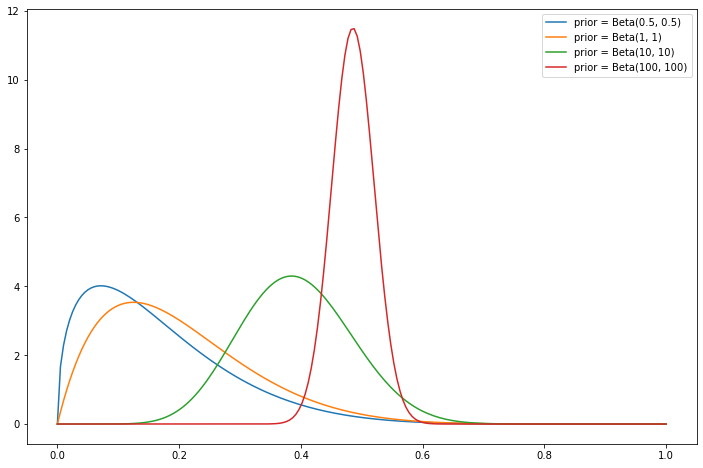
\includegraphics{Figure-12-06}
\end{figure}

    

\textbf{Exercise 12.11.6}. Let
\(X_{1}, \dots, X_{n} \sim \text{Poisson}(\lambda)\).
\textbf{(a)} Let \(\lambda \sim \text{Gamma}(\alpha, \beta)\) be the
prior. Show that the posterior is also a Gamma. Find the posterior mean.
\textbf{(b)} Find the Jeffreys' prior. Find the posterior.

\textbf{Solution}.
\textbf{(a)} The posterior is proportional to the likelihood times the
prior:
\begin{align*}
f(\lambda | X^{n}) &\propto \mathcal{L}(\lambda | X^{n}) f(\lambda) \\
&= \left(\prod_{i=1}^{n} \frac{\lambda^{X_{i}}e^{-\lambda}}{X_{i}!} \right) \frac{\beta^{\alpha}}{\Gamma(\alpha)}\lambda^{\alpha - 1}e^{-\beta \lambda} \\
& \propto \lambda^{\sum_{i} X_{i}} e^{-n\lambda} \lambda^{\alpha - 1}e^{-\beta \lambda} \\
&= \lambda^{\left(\alpha + \sum_{i} X_{i} \right) - 1} e^{-(\beta + n) \lambda}
\end{align*}
Therefore, the posterior is proportional to a Gamma distribution with
parameters \(\left(\alpha + \sum_{i=1}^{n} X_{i}, \beta + n\right)\) -- and
thus it must be drawn from that distribution.
\[
\lambda | X^{n} \sim \text{Gamma}\left(\alpha + \sum_{i=1}^{n} X_{i}, \beta + n \right)
\]
The posterior mean is the mean of Gamma distribution it is drawn from,
\[
\bar{\lambda} | X^{n} = \frac{\alpha + \sum_{i=1}^{n} X_{i}}{\beta + n}
\]
\textbf{(b)} For a Poisson distribution, the log likelihood is
\begin{align*}
\ell_{n}(\lambda) &= \sum_{i=1}^{n} \log \left( \frac{\lambda^{X_{i}} e^{-\lambda}}{X_{i}!}\right)  \\
&= \sum_{i=1}^{n} \left( X_{i} \log \lambda - \lambda - \log (X_{i}!)\right) \\
&= \log \lambda \left( \sum_{i=1}^{n} X_{i} \right) - n\lambda - \sum_{i=1}^{n} \log (X_{i}!)
\end{align*}
Its second derivative is
\(\ell_{n}''(\lambda) = -n \bar{X} / \lambda^{2}\), so Fisher's
information is
\(I(\lambda) = -\EXP[\ell''(\lambda)] = 1 / \lambda\).
Jeffreys' prior is:
\[
f(\lambda) \propto I(\lambda)^{1/2} = \lambda^{-1/2}
\]
The posterior is proportional to the likelihood times the prior:
\begin{align*}
f(\lambda | X^{n}) &\propto \mathcal{L}(\lambda | X^{n}) f(\lambda) \\
&\propto \left(\prod_{i=1}^{n} \frac{\lambda^{X_{i}}e^{-\lambda}}{X_{i}!} \right) \lambda^{-1/2} \\
&\propto \lambda^{\left(1/2 + \sum_{i} X_{i} \right) - 1} e^{-n\lambda}
\end{align*}
Therefore, the posterior is proportional to a Gamma distribution with
parameters \(\left(\left(1/2 + \sum_{i=1}^{n} X_{i} \right), n\right)\) --
and thus it must be drawn from that distribution.
\[
\lambda | X^{n} \sim \text{Gamma}\left(\frac{1}{2} + \sum_{i=1}^{n} X_{i}, n \right)
\]
